\documentclass[10pt,a4paper]{article}
\usepackage[polish]{babel}
\usepackage[utf8]{inputenc}
\usepackage{polski}
\usepackage{indentfirst}
\usepackage{mathtools} 
\usepackage[a4paper,margin=2cm]{geometry}
\usepackage{tabularx}
\usepackage{graphicx}
\usepackage{float}

\usepackage[hidelinks]{hyperref}

\usepackage{amsmath}
\usepackage{algorithm}
\usepackage[noend]{algpseudocode}

\frenchspacing

\usepackage{titlesec}
\titlelabel{\thetitle.\quad}

\begin{document}
	\title{Kryptografia - projekt  \\  Algorytm RSA}
	\author{Piotr Janus, Kamil Piszczek}
	\date{}
	\maketitle

\section{Opis metody}
Algorytm RSA jest jednym z pierwszych praktycznych kryptosystemów korzystających z koncepcji klucza publicznego i jest on powszechnie stosowany do zabezpieczenia transmisji danych. W tym kryptosystemie, klucz szyfrujący jest publiczny i różni się od klucza deszyfrującego, który jest tajny. Ta asymetria kluczy wynika z~faktu, że niezwykle trudno jest rozłożyć na czynniki iloczyn dwóch bardzo dużych liczb pierwszych. 

Nazwa algorytmu RSA pochodzi od pierwszych liter nazwisk jego twórców - Ron Rivesta, Adi Shamira oraz Leonarda Adlemana, którzy po raz pierwszy opisali go w 1977r.

Algorytm RSA jest stosunkowo wolnym algorytm i z tego powodu jest on rzadziej używany do bezpośrednio szyfrowania danych użytkownika. W większości przypadków, przy pomocy RSA przekazywane są klucze do symetrycznych algorytmów szyfrujących, które potem mogą być wykorzystywane do stosunkowo bezpiecznej wymiany danych z dużo wyższą prędkością.

\subsection{Generacja kluczy} \label{key_gen}

Zarówno klucz prywatny jak i publiczny, które wykorzystywane są w algorytmie RSA tworzone są według poniższej procedury:

\begin{enumerate}
\item Wybierz dwie różne liczby pierwszy $p$ oraz $q$.
\item Oblicz $n = pq$. $n$ jest modułem (ang. modulus) zarówno klucza prywatnego jak i publicznego. Oznacza również ich długość (zazwyczaj podawana w bitach).
\item Oblicz funkcję Eulera - tzw. tocjent: $\phi(n) = \phi(p) \phi(q) = (p-1)(q-1)$
\item Wybierz liczbę $e$ taką że: $1<e<\phi(n)$ oraz $NWD(e,phi(n))=1$.
\item Ustal liczbę $d$ taką że:
\begin{equation} \label{ed_cond_eq}
d e \equiv 1 \mod \phi(n).
\end{equation}
\end{enumerate}

Klucz publiczny definiowany jest jako para liczb $(n, e)$, gdzie $n$ to moduł klucza, natomiast $e$ to jego wykładnik.

Klucz prywatny definiowany jest analogicznie jako para liczb $(n, d)$, gdzie $n$ to moduł klucza, natomiast $d$~to jego wykładnik.

\subsection{Szyfrowanie i deszyfrowanie} \label{encode_decode}
Załóżmy, że chcemy zaszyfrować wiadomość $M$. Na początku dzielimy ją na mniejsze $m$ bloki według łatwego do odwrócenia schematu. Następnie obliczamy wartość zaszyfrowanej wiadomości $c$ według wzoru:
\begin{equation} \label{encode_eq}
c \equiv m^e \mod n
\end{equation} 

Załóżmy, że chcemy odszyfrować szyfrogram $c$ i odzyskać wiadomość $m$. Obliczamy wartość odszyfrowanego fragmentu wiadomości według wzoru:
\begin{equation} \label{decode_eq}
m \equiv c^d \mod n
\end{equation}

\subsection{Prosty przykład}

Postępujemy według przepisu \ref{key_gen}:

\begin{enumerate}
\item $p = 61$ oraz $q = 53$.
\item $n = 61 \times 53 = 3233 $.
\item $\phi(3233) = (61-1)(53-1) = 3120$.
\item $e=17$, ponieważ $1<17<3120$ oraz $NWD(3120, 17) = 1$.
\item $d=2753$, ponieważ $2753 \times 17 \equiv 1 \mod 3120$.
\end{enumerate}

Publiczny klucz to para: $(n, e)=(3233,17)$.
Prywatny klucz to para: $(n, e)=(3233,2753)$.

Szyfrogram dla wiadomości $m = 65$ obliczamy z podanego wzoru (\ref{encode_eq}):
\begin{equation} 
m^e = 65^{17} \equiv 2790 \mod 3233
\end{equation}

Oryginalną wiadomość możemy odszyfrować za pomocą wzoru (\ref{decode_eq}):
\begin{equation} 
c^d = 2790^{2753} \equiv 65 \mod 3233
\end{equation}

\subsection{Dowód poprawności}
Dowód poprawności algorytmu RSA opiera się na małym twierdzeniu Fermata. Jeżeli $p$ jest liczbą pierwszą i $a$ nie jest podzielne przez $p$ to wtedy:

\begin{equation} \label{fermat_eq}
a^{p-1} \equiv 1 \mod p
\end{equation}

Chcemy pokazać, że $m^{ed} \equiv m \mod pq$ dla każdej liczby całkowitej $m$. Zgodnie z wcześniejszymi założeniami $p$ oraz $q$ są różnymi liczbami pierwszymi, natomiast $e$ oraz $d$ to liczby całkowite spełniające warunek (\ref{ed_cond_eq}).
Ponieważ: $\phi(pq) = (p-1)(q-1)$, to na mocy (\ref{ed_cond_eq}) możemy stwierdzić, że dla każdego dodatniego i całkowitego $h$ zachodzi równanie:

\begin{equation}  \label{h_cond_eq}
ed-1=h(p-1)(q-1)
\end{equation}

Do zweryfikowania, czy liczby takie jak $m$ czy $m^{ed}$ przystają do siebie modulo $pq$ wystarczy sprawdzić, czy przystają one modulo $p$ oraz modulo $q$ oddzielnie. Wynika to, z chińskiego twierdzenia o reszcie.

Do pokazania, że $m^{ed} \equiv m \mod p$ rozważymy dwa przypadki. 

\begin{enumerate}
\item $m \equiv 0 \mod p$

Wtedy:
\begin{equation} 
m^{ed} \equiv 0 \equiv m \mod p
\end{equation}

\item $m \not\equiv 0 \mod p$

Przekształcamy przy pomocy zależności (\ref{h_cond_eq}) oraz twierdzenia Fermata (\ref{fermat_eq}):

\begin{equation} 
m^{ed} = m^{ed-1}m = m^{h(p-1)(q-1)}m = (m^{p-1})^{h(q-1)}m \equiv 1^{h(q-1)}m \equiv m \mod p
\end{equation}

\end{enumerate}

Analogiczne rozumowanie można przeprowadzić dla czynnika $q$. Te dwie zależności dowodzą poprawności algorytmu RSA:

\begin{equation}
m^{ed} \equiv m \mod pq
\end{equation}


\section{Metody użyte wewnątrz algorytmu}

\subsection{Generacja bardzo dużych liczb pierwszych}

Sprawdzenie czy dana liczba jest pierwsza w przypadku liczb o rozmiarze rzędu kilkuset bitów jest operacją niezwykle złożoną obliczeniowo. W celu optymalizacji stosuje się bardziej zaawansowane testy pierwszości. Przykładem może być test \textit{Millera-Rabina} wykorzystywany w wielu implementacjach.\\ 


\begin{samepage}
\noindent Załóżmy ze chcemy wykonać test na nieparzystej liczbie $n$, metoda składa się z następujących kroków:

\begin{enumerate}
\item Zdefiniuj parametr $k$ określający dokładność testu (zazwyczaj przyjmuje się $k=100$).
\item Wyznacz maksymalną potęgę dwójki dzielącą $n-1$ i zastosuj równość $n-1 = 2^s \cdot d$.
\item {Powtórz $k$ razy:
	\begin{itemize}
		\item wybierz losowe $a$ ze zbioru $\{1,2,\ldots,n-1\}$
		\item jeżeli $a^d \not\equiv 1$ i $a^{2rd} \not\equiv -1 \mod n$ dla każdego $r$ ze zbioru $\{1,2,\ldots,s-1\}$ badana liczba jest \textbf{złożona}
	\end{itemize}
	}
\item Test przeszedł pomyślnie, badana liczba jest \textbf{prawdopodobnie pierwsza}
\end{enumerate}

\end{samepage}

\noindent W przypadku przedstawionej metody, prawdopodobieństwo, że liczba złożona zostanie zaklasyfikowana jako pierwsza wynosi $4^{-k}$.

\subsection{Odwrotność modulo} \label{mod_inv}
Podczas operacji generowania kluczy (sekcja \ref{key_gen}) konieczne jest wyznaczenie liczby całkowitej $x$ spełniającej następujący warunek:

\begin{equation} 
\label{mod_mul_inv1}
a \equiv x^{-1} \mod n
\end{equation}

Równanie to może zostać przekształcone do następującej postaci:

\begin{equation}
\label{mod_mul_inv2}
ax \equiv 1 \mod n
\end{equation}

Problem ten może zostać sprowadzony do \textit{Rozszerzonego Algorytmu Euklidesa}, który wyznacza liczby $x$ i $y$ z następującego równania:

\begin{equation}
\label{extended_euclidean}
ax + by = gcd(a,b)
\end{equation}

Równanie (\ref{mod_mul_inv2}) może zostać doprowadzone do powyższej postaci poprzez następujące przekształcenia:

\begin{equation}
ax - 1 = qn
\end{equation}
\begin{equation}
ax - qn = 1
\end{equation}

Powyższe równanie ma postać zgodną ze wzorem (\ref{extended_euclidean}), w tym przypadku dane jest $a$ oraz $n$, natomiast niewiadomymi są $x$ i $q$. Należy zwrócić uwagę, że do rozwiązania problemu (\ref{mod_mul_inv1}) konieczna jest tylko wartość $x$.\\

Pierwszym krokiem \textit{Rozszerzonego Algorytmu Euklidesa} jest zdefiniowanie następujących oznaczeń:

\begin{center}
$r_{0} = a \quad r_{1} = b$\\
$s_{0} = 1 \quad s_{1} = 0$\\
$t_{0} = 0 \quad t_{1} = 1$
\end{center}

Kolejne iteracje przebiegają następująco:

\begin{center}
$r_{i+1} = r_{i-1} - q_{i} r_{i} = b$\\
$s_{i+1} = s_{i-1} - q_{i} s_{i} = 0$\\
$t_{i+1} = t_{i-1} - q_{i} t_{i} = 1$
\end{center}

Gdzie $q_i$ definiujemy jako iloraz liczb $r_{i-1}$ oraz $r_i$. Warunkiem stopu jest $r_{k+1} = 0$, w takim przypadku szukane wartości $x$ i $y$ to odpowiednio $s_k$ oraz $t_k$. 
 
\subsection{Największy wspólny dzielnik dla dużych liczb}
Największy wspólny dzielnik liczb $a$ i $b$ oznaczany jako $gcd(a,b)$ może zostać wyznaczony między innymi algorytmem binarnym. Został on wybrany ze względu na łatwość implementacji i wydajność, w przeciwieństwie do innych metod (np. metody Euklidesa) wymaga jedynie dzielenia przez 2. Algorytm został przedstawiony w~postaci pseudokodu (funkcja \hyperref[fun_gcd]{\textit{gcd}}).

\begin{algorithm} \label{fun_gcd}
\begin{algorithmic}[1]
\Function{$gcd$}{$a$, $b$}
\State $d := 0$
\While {($a \mod 2 == 0$) and ($b \mod 2 == 0$)} 
	\State $a : =a/2$
	\State $b : =b/2$
	\State $d : = d + 1$
\EndWhile

\While {$a \neq b$} 
	 \If{$a \mod 2 == 0$} \State {$a := a/2$} 
	 \ElsIf{$b \mod 2 == 0$} \State{$b := b/2$} 
	 \ElsIf{$a > b$} \State{$a := (a - b)/2$}
	 \Else \State{$b := (b - a)/2$}
	 \EndIf
\EndWhile

\State \Return {$a \cdot 2^d$}
\EndFunction
\end{algorithmic}
\end{algorithm}


\subsection{Operacja szyfrowania}

Zgodnie z opisem w sekcji \ref{encode_decode} szyfrowanie polega na przeprowadzeniu operacji:
\begin{equation}
c \equiv b^e \mod m
\end{equation}

W celu poprawienia wydajności można do tego celu użyć metody binarnej, która została przedstawiona postaci pseudokodu (funkcja \hyperref[fun_modPow]{\textit{modPow}}).


\begin{algorithm} \label{fun_modPow}
\begin{algorithmic}[1]
\Function{$modPow$}{$b$, $e$, $m$}
\If{$m == 1$} 
	\State {\Return {$0$}} 
\EndIf

\State $res := 1$
\State $b := b \mod m$
\While {$e > 0$} 
	\If{$e \mod 2 == 1$} 
	\State {$res := (res \cdot b) \mod m$} 
	\EndIf
	\State {$e := e/2$}
	\State {$b := (b \cdot b) \mod m$}
\EndWhile

\State \Return {$res$}
\EndFunction
\end{algorithmic}
\end{algorithm}

\subsection{Operacja deszyfrowania}

Podobnie jak operacja szyfrowania, także operacja deszyfrowania w przypadku dużych liczb może być bardzo złożona obliczeniowo. Jedną z możliwości jest wykorzystanie metody analogicznej jak przy szyfrowaniu. Warto zwrócić uwagę, że w przypadku deszyfrowania znamy liczby $p$ i $q$ które zostały wykorzystane do generacji kluczy (sekcja \ref{key_gen}). Obliczenia mogą zostać dodatkowo przyspieszone poprzez wykorzystanie \textit{Chińskiego twierdzenia o resztach}, przyjmując oznaczenia jak w sekcji \ref{encode_decode} możemy odczytać wiadomość $m$ stosując następujące przekształcenia:\\
\\
$d_p = d \mod (p-1)$\\ 
$d_q = d \mod (q-1)$\\
$q_{inv} = q^{-1} \mod p$\\ \\ 
$m_1 = c^{d_p} \mod p$\\
$m_2 = c^{d_q} \mod q$\\
$h = (q_{inv} \cdot (m_1 - m_2)) \mod p$\\
$m = m_2 + h \cdot q$\\

Do obliczenia wartości $q_{inv}$ możemy użyć metody opisanej w sekcji \ref{mod_inv}, natomiast wartości $m_1$ oraz $m_2$ mogą zostać wyznaczone przy pomocy metody binarnej opisanej w poprzednie sekcji.


\section{Implementacja}
\subsection{Użyty język i biblioteki}

Implementacja algorytmu RSA została wykonana w języku \textit{JAVA}, napisany program umożliwia przesyłanie zaszyfrowanych wiadomości tekstowych pomiędzy dwoma komputerami. Do obliczeń matematycznych wykorzystano bibliotekę \textit{BigInteger}, która daje możliwość operowania na bardzo dużych liczbach całkowitych (o~szerokości kilkuset bitów). Komunikacja odbywa się z wykorzystaniem protokołu \textit{TCP IP}. Graficzny interfejs użytkownika został wykonany w technologi \textit{JavaFX}. Dzięki zastosowanemu podejściu, program jest uniwersalny i może zostać z łatwością uruchomiony na każdym systemie operacyjnym. 

\subsection{Funkcjonalność}

Jak zostało wspomniane w poprzednim podpunkcie, aplikacja służy do przesyłania wiadomości tekstowych. Jej działanie może zostać przetestowane poprzez uruchomienie na dwóch komputerach znajdujących się w jednej sieci lub z wykorzystaniem jednego komputera i lokalnego hosta (dokładny opis w rozdziale \ref{subsec:manual}). 

Program może zostać uruchomiony w trybie klienta lub serwera, przesyłanie wiadomości jest możliwe oczywiście w obu kierunkach. Dodatkowo w każdym kierunku komunikacji mamy możliwość określenia innej długości klucza szyfrującego. Po nawiązaniu połączenia następuje generacja klucza publicznego i prywatnego po obu stronach, następnie strony wymieniają się kluczami publicznymi. Od tego momentu zarówno serwer jak i klient mogą przesyłać szyfrowane wiadomości. 

W sekcji \ref{encode_decode} został przedstawiony schemat szyfrowania pojedynczego bloku danych, w przypadku napisanej aplikacji istnieje możliwość wysyłania wiadomości tekstowych o dowolnej długości. Napisany tekst jest dzielony na równe bloki (ostatni jest oczywiście dopełniany zerami), długość takiego bloku jest na nowo losowana dla każdej kolejnej wiadomości. Podczas szyfrowania zgodnie ze wzorem (\ref{encode_eq}) konieczne jest dodatkowo dopełnienie otrzymanej wartości zerowymi bitami tak, aby jej długość była równa długości klucza $n$ (sekcja \ref{key_gen}). Dzięki temu każdy zaszyfrowany blok ma identyczną długość i zaszyfrowana wiadomość może być łatwo podzielona przez odbiorcę.

W oknie aplikacji oprócz podglądu wiadomości w postaci normalnego tekstu, dostępna jest także jej zakodowana postać (w tym przypadku wiadomość jest wyświetlana jako ciąg bajtów). Dodatkowo w oknie komunikatów wyświetlane są informacje o przychodzących i wysyłanych wiadomościach oraz klucze wykorzystywane do szyfrowania. 

\subsection{Manual}
\label{subsec:manual}

\begin{figure}[!h]
	\centering
	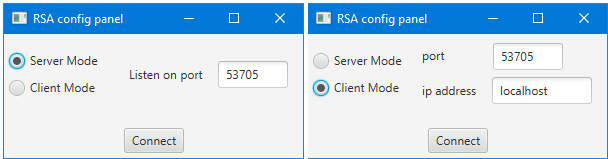
\includegraphics[scale=0.85]{img/config_panel.png}
	\caption{Panel Konfiguracyjny w zależności od wybranego trybu}
	\label{fig:config_panel}
\end{figure}

W celu przetestowania aplikacji należy postępować zgodnie z poniższą instrukcją:

\begin{enumerate}
\item Program należy uruchomić (plik \textit{rsa.jar}) na dwóch komputerach znajdujących się w jednej sieci lub dwa razy na jednym komputerze (okno aplikacji nie jest zbyt duże, zatem bez problemu można operować na dwóch jednocześnie).

\item Po uruchomieniu ukaże nam się ekran przedstawiony na rysunku \ref{fig:config_panel}. Najpierw w jednej aplikacji wybieramy \textit{Server Mode} i naciskamy \textit{Connect}, następnie drugą aplikacje uruchamiamy w trybie \textit{Client Mode}.

\item Po tej czynności ukaże nam się główne okno programu (rysunek \ref{fig:main_window}). W polu na dole powinien pojawić się komunikat o pomyślnym nawiązaniu połączenia. W tym momencie należy w obu aplikacjach zdefiniować długość klucza i nacisnąć przycisk \textit{Start}.

\item Gdy w oknie komunikatów obu aplikacji pojawi się informacja o wygenerowaniu kluczy oraz o otrzymaniu klucza publicznego od drugiego użytkownika (rysunek \ref{fig:key_gen}), możemy przejść do wysyłania i odbierania wiadomości. W celu wysłania wiadomości należy wpisać tekst w odpowiednie pole i nacisnąć przycisk \textit{Decode and send}. Następnie można odczytać wysłaną wiadomość w drugiej aplikacji, poprzez naciśnięcie przycisku \textit{Read next message}.
\end{enumerate}

\begin{figure}[!t]
	\centering
	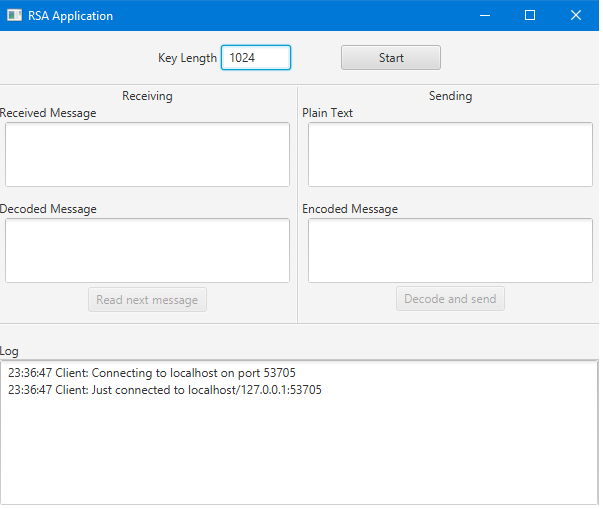
\includegraphics[scale=0.85]{img/main_window.png}
	\caption{Główne okno programu}
	\label{fig:main_window}
\end{figure}

\begin{figure}[!h]
	\centering
	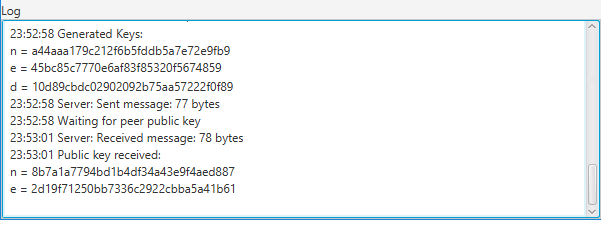
\includegraphics[scale=0.85]{img/key_gen.png}
	\caption{Przykładowy log zawierający informacje o wygenerowanych kluczach}
	\label{fig:key_gen}
\end{figure}

	
\end{document}
